\documentclass[11pt]{article}

\usepackage[utf8]{inputenc}
\usepackage[T1]{fontenc}
\usepackage{mathptmx}
\usepackage[margin=1in]{geometry}
\usepackage[round]{natbib}
\usepackage{url}
\urlstyle{same}
\usepackage{graphicx}
\usepackage{booktabs}
\usepackage{amsmath}
\usepackage[font=small,labelfont=bf]{caption}
\usepackage[hidelinks]{hyperref}

\title{Early Detection of Silent Training Failures in Neural Networks}
\author{Sohan Bhat}
\date{November 2026}

\begin{document}

\maketitle

\begin{abstract}
Neural networks can break during training without raising an error. The run completes and returns a degraded model, and the drop is easy to mistake for a hard problem. This work presents LHD (Layer Health Diagnostics), a monitor that logs four signals for every layer at the end of each epoch (weight change, gradient norm, weight norm, and the fraction of dead units), compares each one with the range it stays within during healthy runs of the same network, flags a layer after three epochs in a row outside that range, names a likely cause, and stops the run. LHD was tested on 645 training runs of a fully connected network on Fashion-MNIST, a CNN on GTSRB, and a small transformer on Tiny Shakespeare, with frozen layers and dead units planted in known layers. LHD caught 411 of 470 broken runs (87\%), named the planted layer in 98\% of the runs it caught, and flagged 3 of 110 fresh healthy runs it had never seen. Averaged within each seed, it was earlier than the accuracy curve for 30 of 30 seed groups, by 9.1 epochs (95\% interval 8.4 to 9.7). A one line check for weights that never change caught all 200 frozen layers two epochs sooner, so LHD's advantage lies in dead units. There, the fixed thresholds used by existing tools either missed most faults or flagged many healthy runs, while LHD caught 78\% of them.
\end{abstract}

\section{Introduction}

During training, neural networks can develop defects, yet nothing fails visibly since the run completes normally and simply produces a degraded result; thus, these are called ``silent failures.'' Because of this, identifying whether the degraded result was caused by a difficult problem or a silent failure becomes difficult; therefore, it is common to misread a failure as normal. I initially encountered this as I was training my small-scale GTSRB (German Traffic Sign Recognition Benchmark) model \citep{stallkamp2012} from scratch, where my model plateaued at 76\%, wasting weeks tuning it, until I found one convolutional layer had been accidentally excluded from the optimizer and was never properly trained. Fixing this minute detail raised the accuracy to 87\%. This is not an isolated case: errors in deep learning implementations rarely cause an exception and instead reveal themselves only through degraded predictive performance \citep{chwilczynski2024}.

Since training runs consume significant compute, every silent failure that goes undetected wastes it. The evidence existed in the form of raw numbers in the weights and biases, but perceiving that is challenging since nothing in standard practice surfaces them. To address this, this work presents LHD (Layer Health Diagnostics), a monitor that reads these numbers, catches the failure within a few epochs, identifies the broken layer and its likely cause, and halts the run before compute is wasted.

LHD was tested on 645 training runs across three networks, with every rule and setting fixed before any broken run was trained. The main findings are the following.

\begin{itemize}
\item LHD caught 411 of 470 runs with a planted frozen layer or dead units (87\%), usually at epoch 3, while the accuracy curve caught 166 of 470 (35\%). LHD was earlier on average for 30 of 30 seed groups and 41 of 47 fault conditions, by 9.1 epochs (95\% interval 8.4 to 9.7).
\item LHD flagged 3 of 110 fresh healthy runs (2.7\%), against 6 of 110 for the accuracy curve.
\item For frozen layers, a check for weights that do not change at all caught 200 of 200 at epoch 1, two epochs before LHD. For dead units, LHD caught 78\% with 3 false alarms, while SageMaker Debugger's default rule caught 53\% and flagged 12 of 110 healthy runs, and stricter defaults from other tools caught almost none.
\item LHD missed small dead unit faults in layers where healthy runs already lose many units, and the planted faults were designed to show up in the signals LHD measures, so these results describe planted faults rather than bugs found in the wild.
\end{itemize}


\section{Related Work}

\paragraph{Karpathy's Recipe.} In 2019, Andrej Karpathy wrote a widely cited guide for the training of neural networks where he discusses how training fails silently \citep{karpathy2019}. He provides manual habits to catch these silent failures, and the Stanford CS231n course notes add checking that the update-to-weight ratio is near 0.1\% \citep{cs231n}. However, his guide simply provides a checklist a human needs to follow by hand with no mention of any automated solution.

\paragraph{wandb.ai.} Weights \& Biases (wandb) is the industry standard for experiment tracking through a dashboard where one line of code in a project can log live gradient and weight histograms during training \citep{biewald2020}. Still, it is limited by only displaying the numbers and nothing more, since a human still needs to watch, understand what healthy numbers look like, and catch the anomaly.

\paragraph{wandb-callbacks.} Wandb-callbacks is a small community add-on package for wandb that includes a dead-ReLU warning callback, which by default warns when at least 80\% of a layer's units never activate \citep{groeger_wandbcallbacks}. However, it covers only one failure mode with a single signal and provides no diagnosis or halting.

\paragraph{DeepLocalize.} DeepLocalize, published at the 2021 International Conference on Software Engineering, watches the values a network produces at each layer during training and, when it finds a numerical error, traces the error back to the layer that caused it \citep{wardat2021}. However, it only reports faults that lead to numerical errors and does not suggest how to fix them \citep{wardat2022}.

\paragraph{UMLAUT.} UMLAUT, presented at the 2021 ACM Conference on Human Factors in Computing Systems, checks a deep learning program's structure and its model's behavior against debugging heuristics drawn from experts, then shows readable error messages next to the code and the model's output in a single interface \citep{schoop2021}. In a study with 15 participants, people using it found and fixed significantly more bugs than without it. Still, its heuristics fire on models with no known bugs, and the authors of DeepDiagnosis observed it warning of possible overfitting on 68 of 78 such MNIST models \citep{wardat2022}.

\paragraph{SageMaker Debugger.} Amazon SageMaker Debugger records tensors during training jobs on Amazon's cloud and checks them with built-in rules such as DeadRelu, VanishingGradient, ExplodingTensor, UnchangedTensor, and WeightUpdateRatio \citep{aws_rules}. Any rule can be paired with an action that stops the training job when the rule fires \citep{aws_actions}, so detection and halting are already automated. However, its dead unit, gradient, and unchanged tensor rules compare a signal against a fixed default threshold. DeadRelu, for example, fires when more than 50\% of a layer's ReLUs are active less than 1\% of the time, and a user training a different network has to pick a new threshold by hand. Its SimilarAcrossRuns rule compares a job with one other completed job rather than with the range seen across many healthy runs. Amazon's documentation also states that Debugger is no longer open to new customers.

\paragraph{AutoTrainer.} AutoTrainer is a training monitor and automatic repair system published at the 2021 International Conference on Software Engineering \citep{zhang2021}. During training, it checks gradients, weights, and the loss and accuracy curves against preset thresholds to detect five problems: vanishing gradients, exploding gradients, dying ReLU, oscillating loss, and slow convergence. When it finds one, it retrains the model with built-in fixes such as replacing the activation function, adding batch normalization, or changing the weight initializer. However, it does not report which layer is at fault \citep{wardat2022}, and its default thresholds are the same for every network. A later study of model repair on 9 real and 21 artificial faulty models found that a random search did as well as or better than AutoTrainer and two hyperparameter tuning methods, and that all of them failed on larger models \citep{kim2023}.

\paragraph{DeepDiagnosis.} DeepDiagnosis, published at the 2022 International Conference on Software Engineering, checks a model at the end of every training epoch for eight error symptoms, including dead nodes, unchanged weights, saturated activations, and vanishing or exploding gradients \citep{wardat2022}. When it finds a symptom, it reports the layer, maps the symptom to a likely root cause, and suggests a fix, which is close to the layer, cause, and suggested check that LHD reports. However, its checks also rely on fixed thresholds, such as counting a layer as having dead nodes when more than 70\% of its ReLU units are inactive. On 188 models from the AutoTrainer benchmark with no known bugs, it still reported symptoms, including dead nodes in 21 of the 35 CIFAR-10 models \citep{wardat2022}.

\paragraph{ART.} Actually Robust Training is a Python library inspired by Karpathy's recipe that adds validation checks to training pipelines \citep{chwilczynski2024}. While this is a step up, it only imposes process steps at development time rather than live fault detection from internal signals during training.

\medskip

To conclude, tools that detect faults during training, and even stop or repair the run, already exist. However, their dead unit and gradient checks compare each signal against a threshold chosen in advance, such as 50\%, 70\%, or 80\% of a layer's units being dead, even though the share of units that die during healthy training differs between networks and between layers. A threshold that suits one network can therefore miss real faults in another or flag its healthy runs, as DeepDiagnosis's dead node check did on CIFAR-10 models with no known bugs. LHD instead measures a separate healthy range for every layer, signal, and epoch from healthy runs of the network being trained. Furthermore, DeepDiagnosis is evaluated by how many buggy models it flags and how quickly, not by how many epochs earlier its signals catch a fault than the accuracy curve or by how often it flags fresh healthy runs of the same network, and those are the two measurements this work reports.



\section{Method}

\subsection{Signals}

At the end of every epoch, LHD records four signals for each watched layer. Let $W_e$ be the layer's weights and bias at the end of epoch $e$, flattened into one vector, and $\lVert \cdot \rVert$ the square root of the sum of squared entries.

\begin{itemize}
\item \textbf{Weight change} is $\lVert W_e - W_{e-1} \rVert / \lVert W_{e-1} \rVert$, how far the weights moved during the epoch relative to their size. A frozen layer reads exactly 0.
\item \textbf{Weight norm} is $\lVert W_e \rVert$, which grows past normal before a run diverges.
\item \textbf{Gradient norm} is the mean of $\lVert \partial L / \partial W \rVert$ over the epoch's batches, measured after each backward pass and before the optimizer step. A vanishing gradient reads near 0.
\item \textbf{Dead unit fraction} is the share of the layer's units whose output after the ReLU is exactly 0 for every input in a fixed probe batch of 256 validation examples. A unit is one neuron of a dense layer or one filter of a convolution, and a filter counts as dead only when it outputs 0 at every position.
\end{itemize}

The probe batch is the same in every run and is passed through the network in evaluation mode without gradients.

\subsection{Healthy range}

The healthy range is measured only on calibration runs, trained with no defects from different random starting points. For layer $\ell$, signal $s$, and epoch $e$, let $a_{\ell s e}$ and $b_{\ell s e}$ be the lowest and highest values across the calibration runs. A value $x$ is out of range when
\begin{equation}
x < a_{\ell s e}(1 - m) \quad \text{or} \quad x > b_{\ell s e}(1 + m) + f,
\end{equation}
with margin $m = 0.5$ and floor $f = 0.05$, and a value that is not a finite number is always out of range. The floor keeps a signal that is 0 in every healthy run, such as the dead unit fraction of most layers, from flagging a single unusual unit. Broken runs are never used to set the range, because a detector tuned on a known fault only catches that fault. Figure~\ref{fig:healthy_band_cnn} shows the range for one CNN layer.

\begin{figure}[t]
\centering
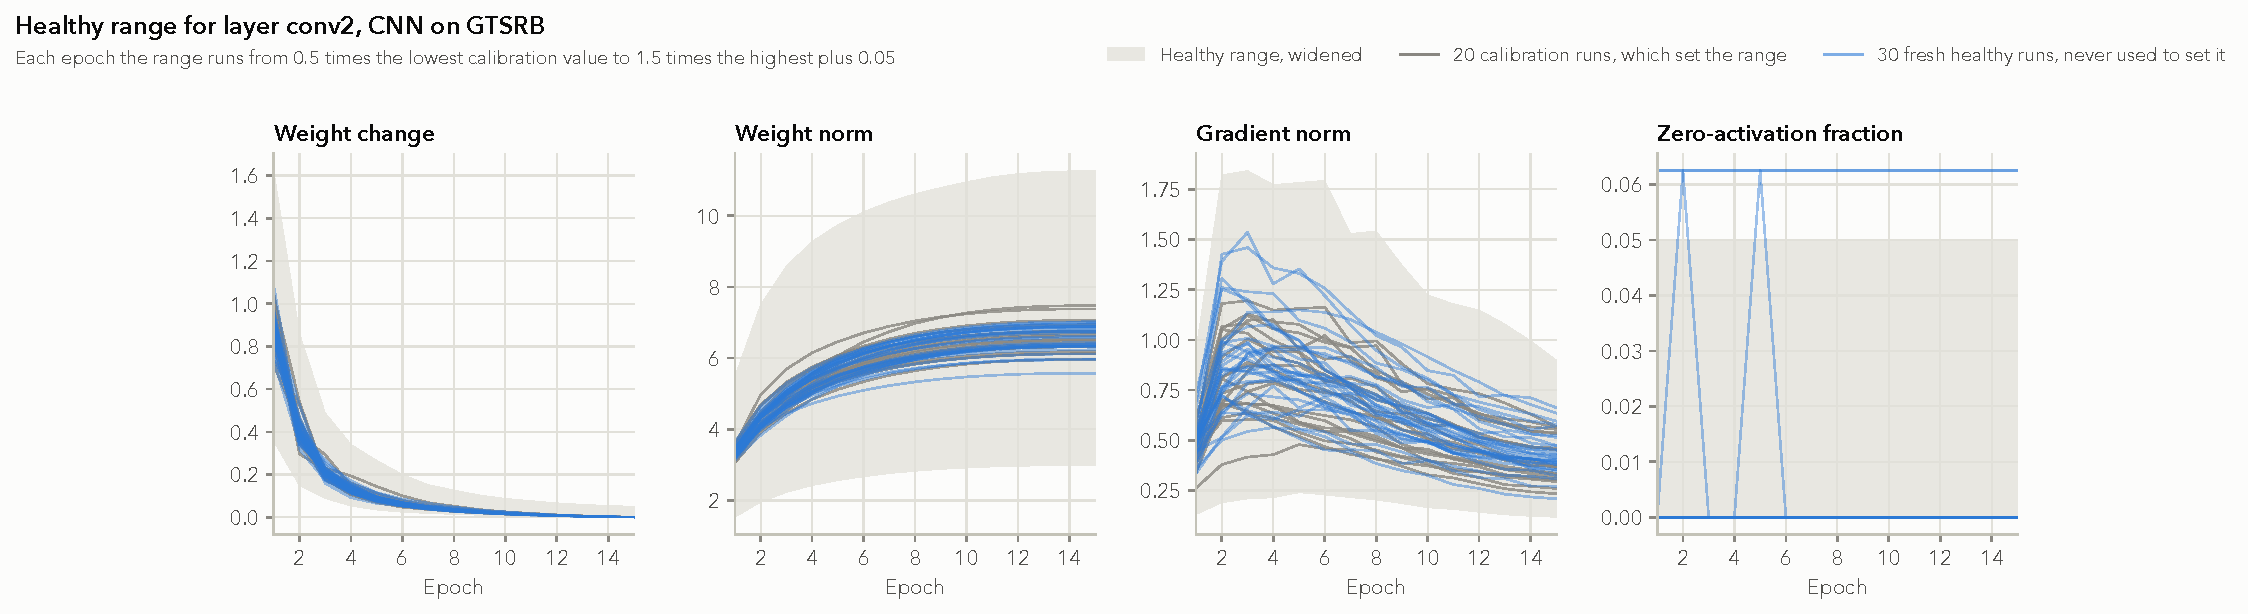
\includegraphics[width=\linewidth]{figures/healthy_band_cnn.pdf}
\caption{The healthy range for the CNN layer conv2. Gray lines are the 20 calibration runs that set the range, blue lines are fresh healthy runs that never touched it, and the shaded band is the range after the margin and floor.}
\label{fig:healthy_band_cnn}
\end{figure}


\subsection{Alarm and diagnosis}

LHD raises an alarm when one signal of one layer stays out of range for $p = 3$ epochs in a row. If several layers reach that point in the same epoch, LHD reports the first one in the order data flows through the network. The settings $m$, $f$, and $p$ were taken from the LHD library's own tests and fixed before any broken run was trained. LHD then names a likely cause from the pattern across the alarmed layer's four signals (Table~\ref{tab:rules}), stops training, and reports the layer, the signals out of range, the cause, and a suggested check. For a frozen layer, for example, the suggested check is that the layer's parameters are passed to the optimizer.

\begin{table}[t]
\centering
\small
\caption{Rules LHD uses to name a cause, checked in order on the alarmed layer.}
\label{tab:rules}
\begin{tabular}{@{}rll@{}}
\toprule
Order & Pattern & Cause named \\
\midrule
1 & any signal not a finite number & diverged \\
2 & dead unit fraction above range & dead units \\
3 & weight change below range, gradient norm inside or above & frozen layer \\
4 & weight change below range, gradient norm below & vanishing gradient \\
5 & weight norm above range & runaway weights \\
6 & anything else & unrecognized \\
\bottomrule
\end{tabular}
\end{table}


\section{Experimental Setup}

\subsection{Networks and data}

LHD was tested on three networks with different structures (Table~\ref{tab:networks}). The fully connected network has hidden layers of 256, 128, and 64 units. The CNN has three convolutions with 8, 16, and 32 filters, each followed by a ReLU and max pooling, then a dense layer of 64 units and the output layer. The transformer predicts the next character with a width of 64, 4 attention heads, 2 blocks, and a ReLU feed-forward layer of 256 units, so dead units can be counted the same way in every network. Validation accuracy is measured on each dataset's test split after every epoch. The CNN is scored on a fixed random subset of 4,000 test images, and the transformer on 512 fixed windows of 64 characters from the last 10\% of the text.

\begin{table}[t]
\centering
\small
\caption{Networks, datasets, and training settings. Training examples for the transformer count characters.}
\label{tab:networks}
\begin{tabular}{@{}llrrrrrr@{}}
\toprule
Network & Dataset & Parameters & Watched layers & ReLU layers & Epochs & Batch & Training examples \\
\midrule
Fully connected & Fashion-MNIST & 242,762 & 4 & 3 & 20 & 128 & 60,000 \\
Transformer & Tiny Shakespeare & 112,577 & 11 & 2 & 15 & 32 & 1,003,854 \\
CNN & GTSRB & 41,659 & 5 & 4 & 15 & 128 & 26,640 \\
\bottomrule
\end{tabular}
\end{table}

Every run used Adam with a learning rate of 0.001 and a cosine schedule, on one CPU thread. The seed fixes both the starting weights and the order of training batches, so a broken run and the healthy run with the same seed differ only by the fault. That healthy run is the broken run's twin, and the twin's final accuracy shows what the fault cost.

\subsection{Planted faults}

Each broken run has one fault planted in one layer at the start of training. A frozen layer has its weights and bias restored after every optimizer step, so gradients are computed but never applied, the same failure as a layer left out of the optimizer. Dead units are made by setting the incoming weights of 10\%, 25\%, or 50\% of a layer's units to 0 and their bias to $-1$, so their ReLU output is 0 for every input, and the optimizer's running averages for those units are cleared. Frozen layers were planted in every watched layer and dead units in every layer followed by a ReLU.

\subsection{Runs}

Calibration runs used seeds 0 to 19 and only set the healthy range. Fresh healthy runs and broken runs used seeds from 1000 up, so no evaluation run touched the range (Table~\ref{tab:runs}). Every run trained for all its epochs, and LHD's alarm was found by replaying the saved signals, which gives the same answer as running LHD live. This let every detector be scored on the same complete runs.

\begin{table}[t]
\centering
\small
\caption{Training runs by role.}
\label{tab:runs}
\begin{tabular}{@{}lrrrr@{}}
\toprule
Network & Calibration & Fresh healthy & Broken & Total \\
\midrule
Fully connected & 20 & 50 & 135 & 205 \\
Transformer & 20 & 30 & 170 & 220 \\
CNN & 20 & 30 & 170 & 220 \\
\bottomrule
\end{tabular}
\end{table}

\subsection{Detectors compared}

The accuracy curve raises suspicion when validation accuracy falls below the lowest calibration value for that epoch 3 epochs in a row, the same patience LHD uses and with no margin, which makes it more sensitive than LHD's rule. A version that needs only one epoch and a loss curve version were also scored. Two kinds of fixed rule that need no healthy runs were added to test whether LHD does better than checks anyone could write by hand. The zero update check fires when some layer's weights do not move at all in an epoch, like SageMaker Debugger's UnchangedTensor rule. The dead unit checks fire when some ReLU layer has at least a fixed share of dead units, at 50\% (the default of SageMaker Debugger's DeadRelu rule), 70\% (DeepDiagnosis), 80\% (the default of wandb-callbacks), or any dead unit at all (its verbose mode). SageMaker counts a ReLU as inactive when it is active less than 1\% of the time, which is close to but not the same as LHD's definition.

\subsection{Measures and statistics}

A broken run is caught when a detector fires at or after the fault's onset, and a false alarm is any alarm on a fresh healthy run. The gap is the accuracy curve's epoch minus LHD's epoch, with ``never'' counted as one epoch past the end of the run. Runs that share a seed share starting weights and batch order, and runs that share a fault and layer share the same break, so single runs are not independent. The main tests therefore average the gap within each seed and within each fault condition, then apply a one sided Wilcoxon signed rank test to those averages, and the 95\% interval for the mean gap comes from a bootstrap with 10,000 draws that resamples whole seeds. Rates are given with 95\% Wilson intervals in the data tables.


\section{Results}

\subsection{Detection and timing}

Table~\ref{tab:headline} gives the main results for each network. Across all three, LHD caught 411 of 470 broken runs and the accuracy curve caught 166 of 470. Of the runs LHD caught, the accuracy curve never noticed 61\%, and 66\% of all broken runs finished with a final accuracy inside the healthy range. LHD's median alarm came at epoch 3, which is the earliest possible alarm for a fault planted at epoch 1 under a patience of 3 epochs. Figure~\ref{fig:cumulative_detection} shows the share of broken runs flagged by each epoch.

Averaged within each seed, LHD was earlier than the accuracy curve for 30 of 30 seed groups ($p = 9.3 \times 10^{-10}$). Averaged within each fault condition, it was earlier for 41 of 47 ($p < 10^{-10}$). The mean gap was 9.1 epochs, with a 95\% interval of 8.4 to 9.7 from the seed bootstrap.

On fresh healthy runs, LHD raised 3 false alarms in 110 runs: one run in the fully connected network's fc2 at epoch 16, where only 1.6\% of units were dead, fewer than in any calibration run (lowest 3.9\%); two runs in the CNN's conv2 at epochs 3 and 4, where 6.2\% of units were dead and no calibration run had a single dead unit there. When no calibration run had a dead unit in a layer, the top of that layer's range is the 0.05 floor, so one dead filter out of 16 is enough to cross it. An alarm for too few dead units does not point to a fault, so checking the dead unit fraction against only the upper end of its range would remove that kind of false alarm.

\begin{figure}[t]
\centering
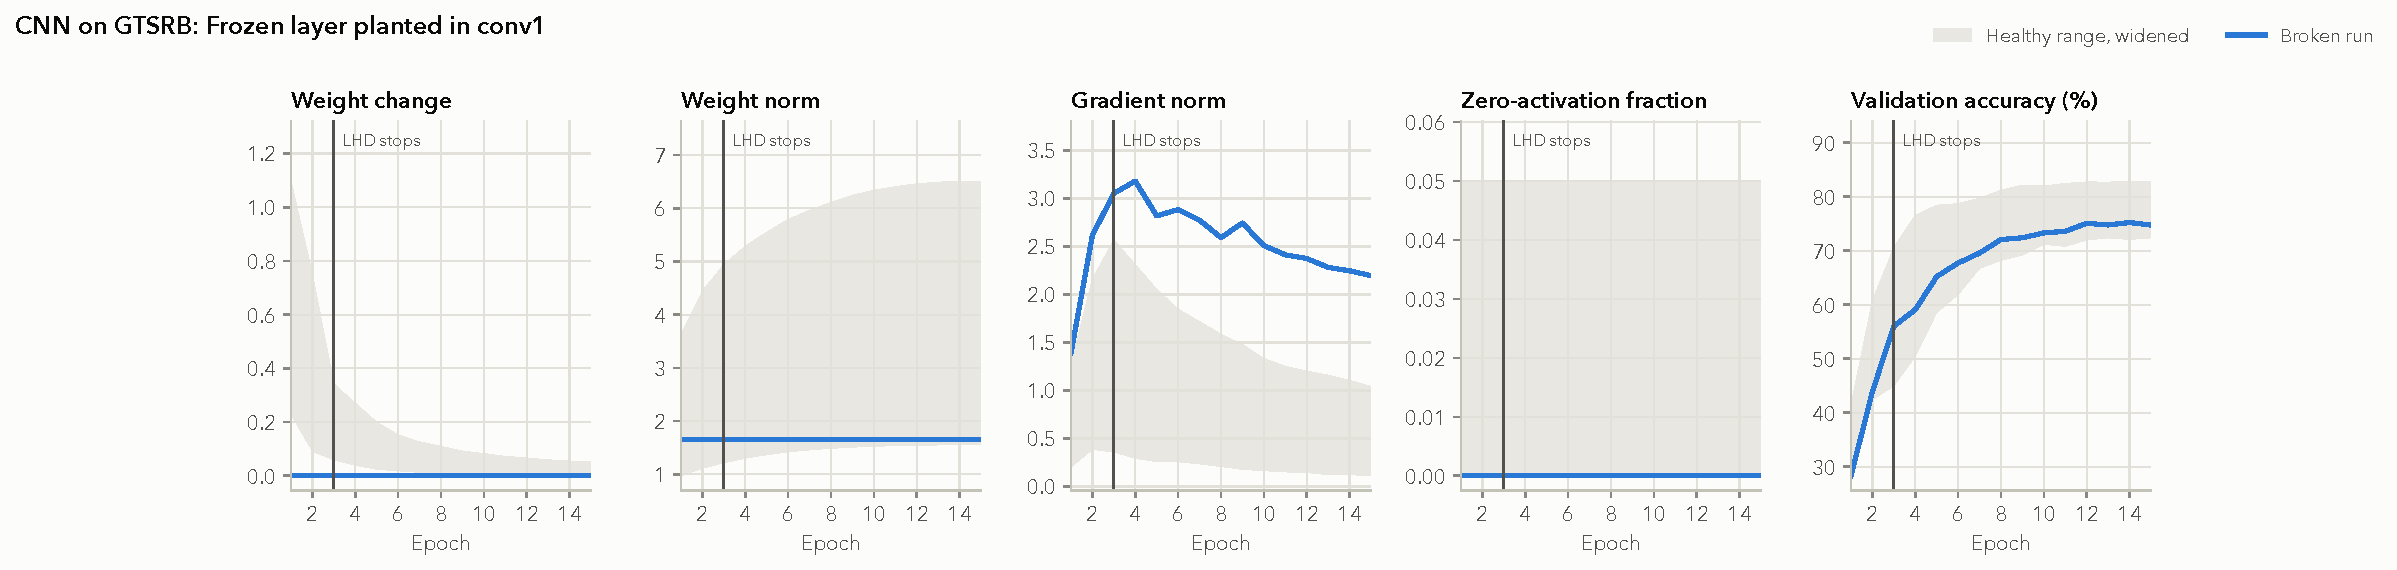
\includegraphics[width=\linewidth]{figures/anatomy_cnn_frozen.pdf}
\caption{One CNN run with a frozen layer. Each panel is one signal of the planted layer against its healthy range, and the last panel is validation accuracy. The vertical rule marks the epoch of LHD's alarm.}
\label{fig:anatomy_cnn_frozen}
\end{figure}


\begin{table}[t]
\centering
\small
\caption{Results on the planted frozen layers and dead units, by network. The gap interval comes from a bootstrap over seeds.}
\label{tab:headline}
\begin{tabular}{@{}lrrr@{}}
\toprule
 & Fully connected & Transformer & CNN \\
\midrule
Broken runs & 130 & 170 & 170 \\
Caught by LHD & 84\% & 100\% & 78\% \\
Right layer, when caught & 100\% & 100\% & 94\% \\
Right cause, when caught & 100\% & 97\% & 94\% \\
Median epoch LHD fired & 3 & 3 & 3 \\
Caught by the accuracy curve & 26\% & 48\% & 29\% \\
Median epoch accuracy curve fired & 17 & 5 & 7 \\
Final accuracy inside healthy range & 69\% & 59\% & 69\% \\
Fresh healthy runs & 50 & 30 & 30 \\
Flagged by LHD & 1 of 50 & 0 of 30 & 2 of 30 \\
Flagged by the accuracy curve & 1 of 50 & 5 of 30 & 0 of 30 \\
Mean epochs LHD was earlier & 12.4 (11.9 to 12.8) & 8.3 (6.4 to 9.8) & 7.4 (6.7 to 8.0) \\
\bottomrule
\end{tabular}
\end{table}

\begin{figure}[t]
\centering
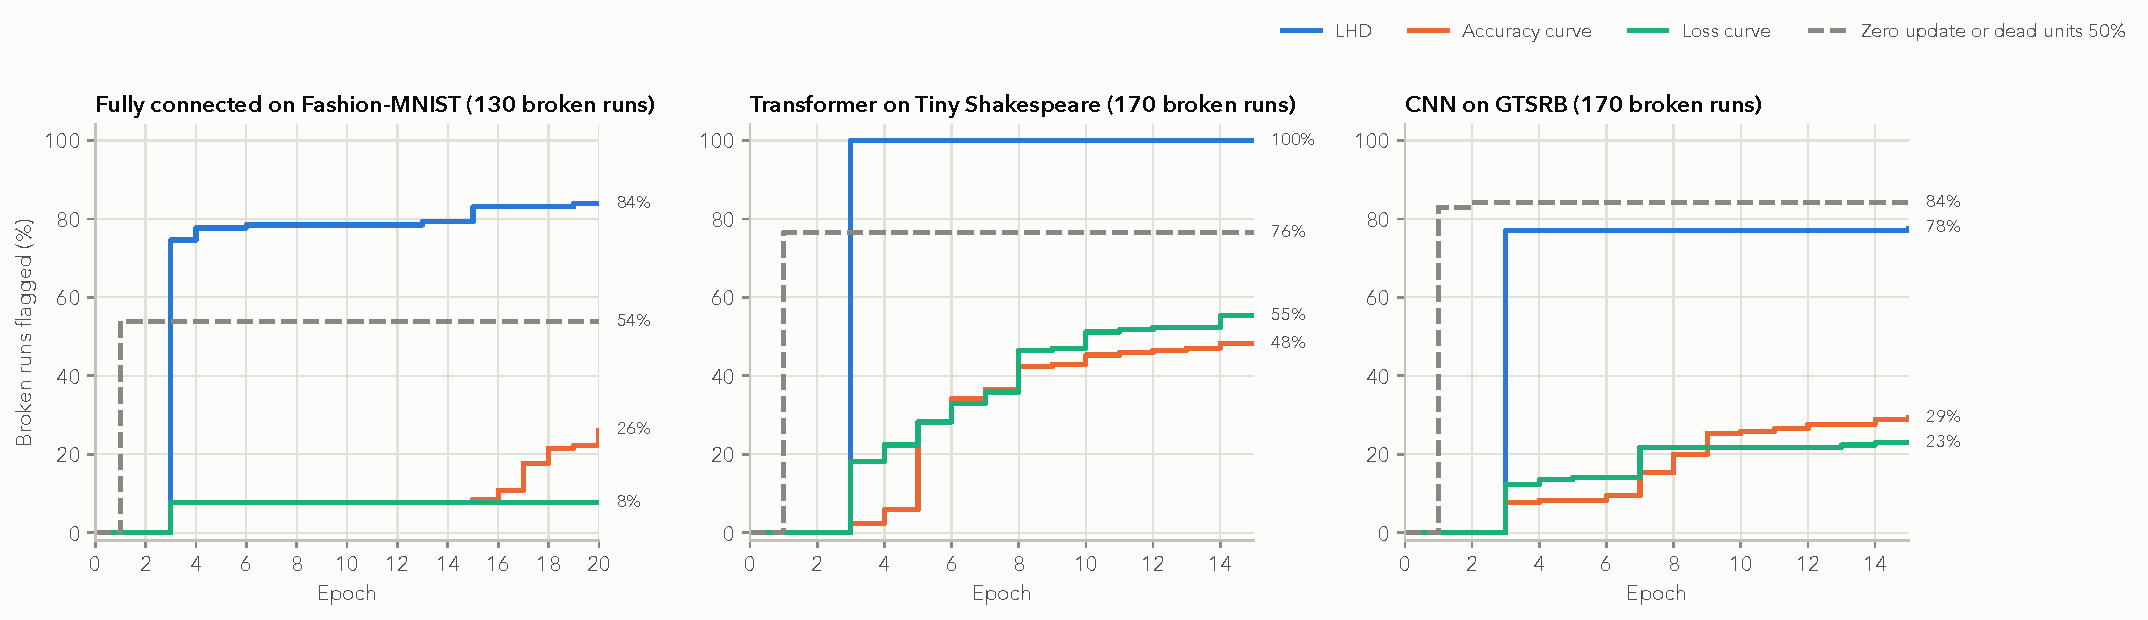
\includegraphics[width=\linewidth]{figures/cumulative_detection.pdf}
\caption{Share of broken runs flagged by each epoch, for LHD, the accuracy curve, the loss curve, and the zero update or 50\% dead unit check.}
\label{fig:cumulative_detection}
\end{figure}


\subsection{Comparison with other detectors}

Table~\ref{tab:detectors} and Figure~\ref{fig:detector_comparison} compare LHD with every other detector on the same runs. For frozen layers, LHD adds nothing over the zero update check, which caught 200 of 200 at epoch 1 with no false alarms, two epochs before LHD. A frozen layer's weight change is exactly 0, so a check for an exact 0 needs no healthy range and no patience.

Dead units are where the healthy range matters. LHD caught 78\% of dead unit faults with 3 false alarms. A fixed rule either missed most faults or flagged many healthy runs. A 25\% rule came closest, catching 83\%, but it flagged 31 of 110 healthy runs, and a rule that fires on any dead unit caught 100\% while flagging 80 of 110. The defaults of SageMaker Debugger, DeepDiagnosis, and wandb-callbacks sit in between. Healthy networks differ in how many units die on their own. In the CNN's dense layer, between 36\% and 70\% of units were dead in healthy calibration runs, while no calibration run of the transformer had more than 0\% dead units in any layer, so no single threshold fits every layer and LHD's per layer range does.

\begin{table}[t]
\centering
\small
\caption{Every detector on the same broken and healthy runs, pooled over the three networks. The median epoch is over the runs each detector caught.}
\label{tab:detectors}
\begin{tabular}{@{}lrrrr@{}}
\toprule
Detector & Frozen caught & Dead units caught & Healthy flagged & Median epoch \\
\midrule
LHD & 100\% & 78\% & 3 of 110 & 3 \\
Accuracy curve, 3 epochs & 63\% & 15\% & 6 of 110 & 6 \\
Accuracy curve, 1 epoch & 86\% & 44\% & 38 of 110 & 3 \\
Loss curve, 3 epochs & 58\% & 10\% & 7 of 110 & 5 \\
Zero update check & 100\% & 0\% & 0 of 110 & 1 \\
Dead units, 25\% & 20\% & 83\% & 31 of 110 & 1 \\
Dead units, 50\% (SageMaker) & 12\% & 53\% & 12 of 110 & 1 \\
Dead units, 70\% (DeepDiagnosis) & 1\% & 4\% & 0 of 110 & 1 \\
Dead units, 80\% (wandb-callbacks) & 0\% & 0\% & 0 of 110 & -- \\
Any dead unit (wandb-callbacks) & 45\% & 100\% & 80 of 110 & 1 \\
\bottomrule
\end{tabular}
\end{table}

\begin{figure}[t]
\centering
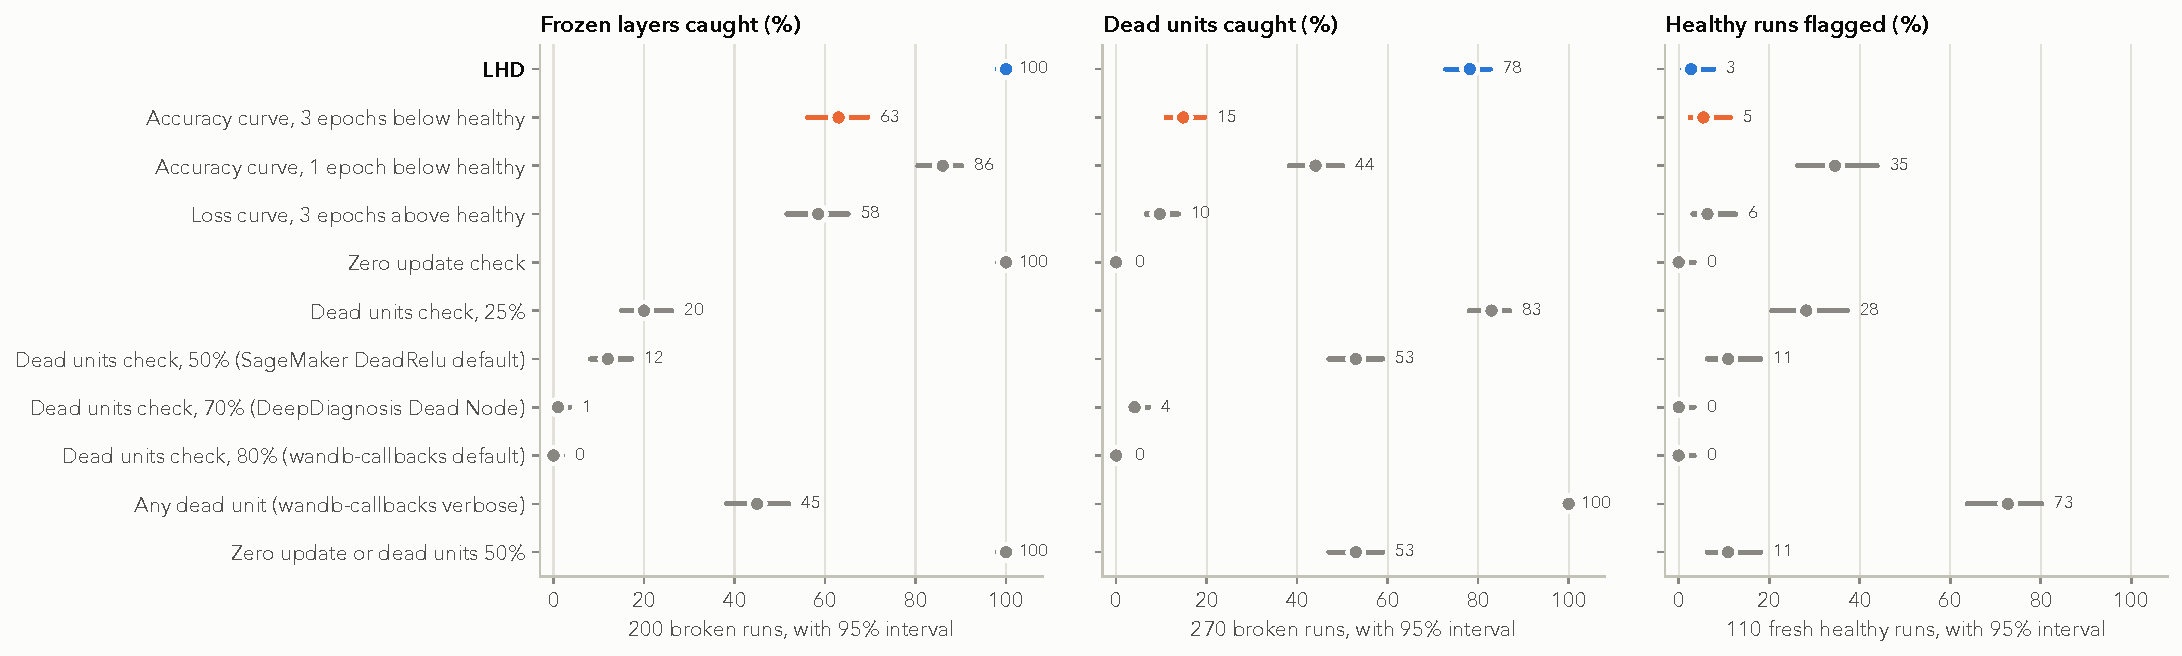
\includegraphics[width=\linewidth]{figures/detector_comparison.pdf}
\caption{Every detector on the same runs, pooled over the three networks, with 95\% Wilson intervals.}
\label{fig:detector_comparison}
\end{figure}


\subsection{How many units must die}

Figure~\ref{fig:dose_response} shows how often LHD and the accuracy curve caught dead unit faults as the killed share grew from 10\% to 50\%. LHD's misses were concentrated in a few layers: CNN conv3 at 10\% (1 of 10 caught), CNN fc1 at 10\% (0 of 10 caught), CNN fc1 at 25\% (0 of 10 caught), CNN fc1 at 50\% (1 of 10 caught), fully connected network fc2 at 10\% (0 of 10 caught), fully connected network fc3 at 10\% (0 of 10 caught), fully connected network fc3 at 25\% (9 of 10 caught). In each of these layers, healthy runs already lose a share of units on their own, so the planted fault stayed inside the healthy range. The CNN's dense layer is the clearest case, since its healthy range already spans most of the planted values.

\begin{figure}[t]
\centering
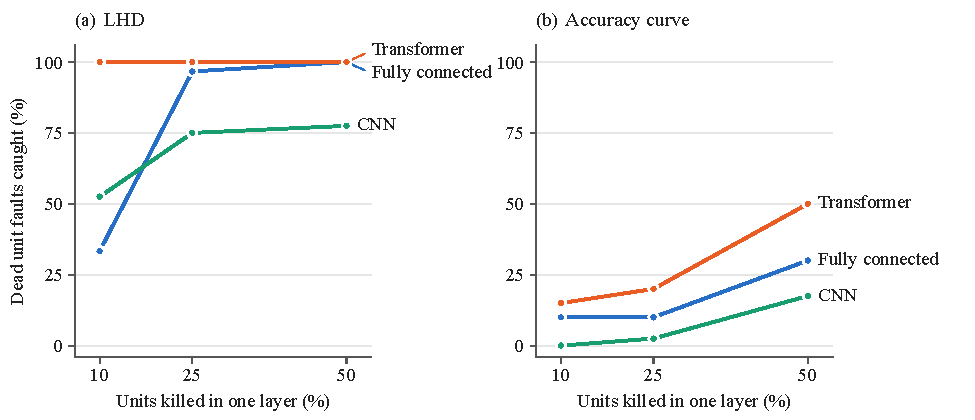
\includegraphics[width=\linewidth]{figures/dose_response.pdf}
\caption{Share of dead unit faults caught as the killed share grows, for LHD and the accuracy curve, by network, with 95\% Wilson intervals.}
\label{fig:dose_response}
\end{figure}


\subsection{Faults that cost accuracy}

Most planted faults did little harm. 223 of 470 broken runs lost under half a point of final accuracy against their healthy twin, and the accuracy curve missing those runs is partly the curve being right. On the 105 runs that lost 2 points or more, LHD caught 94 and the accuracy curve caught 60. Table~\ref{tab:harm} splits broken runs by how much accuracy they lost, and Figure~\ref{fig:accuracy_curves} shows why the accuracy curve struggles. Averaged by fault, broken runs stay inside the healthy accuracy range for most of training. The clearest exception is a frozen layer in the CNN, which cost about as much as the frozen convolution in the GTSRB model that motivated this work.

\begin{table}[t]
\centering
\small
\caption{Broken runs caught, split by accuracy lost against the healthy twin. The simple check is the zero update check or a 50\% dead unit rule.}
\label{tab:harm}
\begin{tabular}{@{}lrrrrr@{}}
\toprule
Accuracy lost & Runs & Mean lost (points) & LHD & Accuracy curve & Simple check \\
\midrule
under 0.5 points & 223 & -0.04 & 83\% & 15\% & 53\% \\
0.5 to 2 points & 142 & 1.00 & 92\% & 51\% & 93\% \\
2 points or more & 105 & 7.22 & 90\% & 57\% & 88\% \\
\bottomrule
\end{tabular}
\end{table}

\begin{figure}[t]
\centering
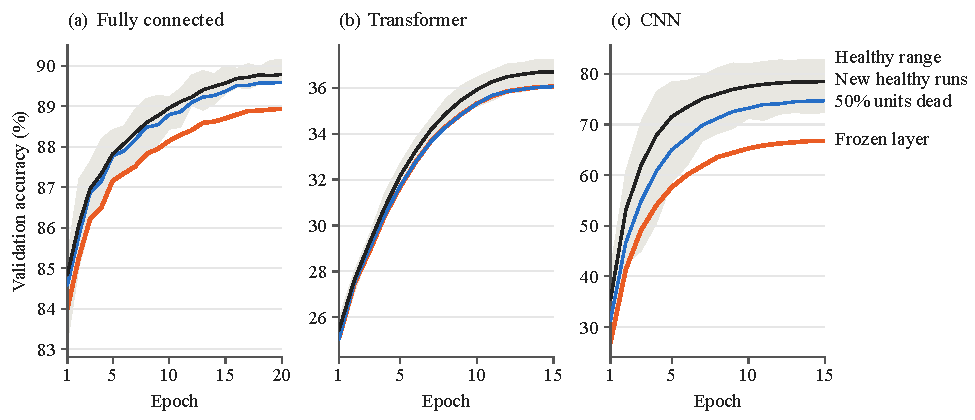
\includegraphics[width=\linewidth]{figures/accuracy_curves.pdf}
\caption{Validation accuracy over training. The shaded band is the range of the calibration runs and the dark line the mean of fresh healthy runs. Colored lines are the mean of broken runs for each fault.}
\label{fig:accuracy_curves}
\end{figure}


\subsection{Diagnosis}

When LHD caught a broken run, it named the planted layer in 98.1\% of cases and the planted cause in 96.8\% (Figure~\ref{fig:per_layer}). It named the wrong layer in 8 caught runs: CNN 50\% dead units in fc1 reported as fc2 (1); CNN frozen conv2 reported as conv1 (1); CNN frozen conv3 reported as conv2 (1); CNN frozen fc1 reported as conv1 (1); CNN frozen fc1 reported as conv2 (1); CNN frozen fc1 reported as conv3 (3). In each case the reported layer's own signal was out of range, dead units in 5 runs and another signal in 3, so LHD found a real effect of the fault in a different layer. In the 7 frozen cases, the planted layer's weight change crossed its range at the same epoch, but when several layers cross at once LHD names the first in data flow order, so reporting every layer out of range would have included the planted one. It named the right layer but the wrong cause in 5 runs: transformer frozen b1.qkv called vanishing gradient (5). A frozen attention projection also lowers the gradient that reaches it, so its pattern matches a vanishing gradient. The high rate of naming the right cause is largely built into the design, since the faults produce exactly the signal patterns the rules look for.

\begin{figure}[t]
\centering
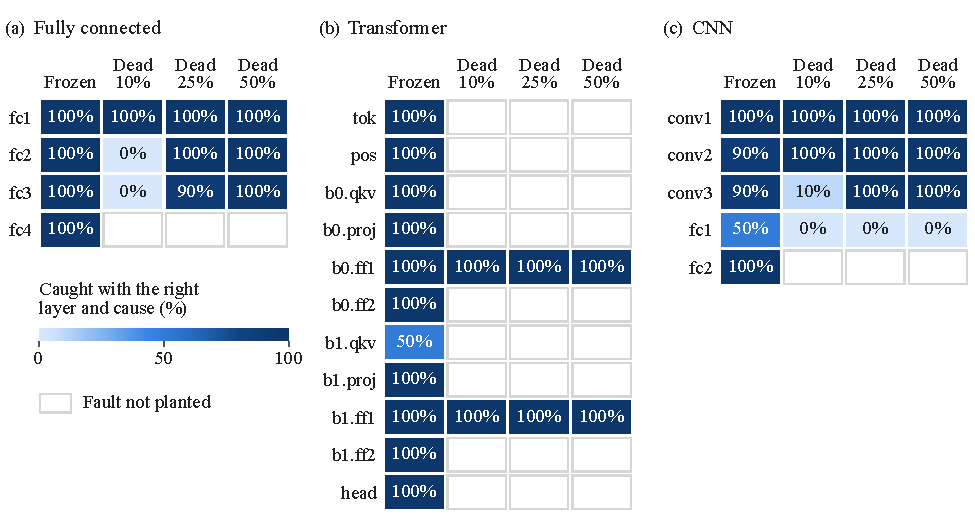
\includegraphics[width=\linewidth]{figures/per_layer.pdf}
\caption{Share of caught runs where LHD named both the planted layer and the right cause, by fault and layer.}
\label{fig:per_layer}
\end{figure}


\subsection{Each signal's part}

Table~\ref{tab:ablation} replays the same runs with signals removed or used alone. The dead unit fraction carries most of the detection, and the weight change is what lets LHD tell a frozen layer apart from other faults. Removing the weight norm or the gradient norm changed little on these faults, which were not designed to move them.

\begin{table}[t]
\centering
\small
\caption{Signal ablation. Each cell gives the percent of broken runs caught, then the percent where LHD named both the right layer and the right cause.}
\label{tab:ablation}
\begin{tabular}{@{}lrrr@{}}
\toprule
Signals used & Fully connected & Transformer & CNN \\
\midrule
all four & 84 / 84 & 100 / 97 & 78 / 73 \\
without weight change & 84 / 53 & 53 / 35 & 75 / 48 \\
without weight norm & 84 / 84 & 100 / 97 & 78 / 73 \\
without grad norm & 84 / 84 & 100 / 100 & 77 / 74 \\
without dead unit fraction & 31 / 31 & 65 / 62 & 30 / 28 \\
only weight change & 31 / 31 & 65 / 65 & 29 / 29 \\
only weight norm & 15 / 0 & 0 / 0 & 16 / 0 \\
only grad norm & 31 / 0 & 18 / 0 & 28 / 0 \\
only dead unit fraction & 70 / 53 & 35 / 35 & 55 / 48 \\
\bottomrule
\end{tabular}
\end{table}

\subsection{Settings and calibration}

Thresholds placed right at the edge of the healthy range flagged many healthy runs. Raising the margin from 0 to 0.5 at a patience of 3 cut false alarms (fully connected network 68\% to 2\%; transformer 80\% to 0\%; CNN 60\% to 7\%), while broken runs caught fell only a little (Figure~\ref{fig:tradeoff}). The healthy range also needs enough calibration runs. Built from 2 runs, it flagged on average fully connected network 22\%, transformer 0\%, CNN 22\% of healthy runs, and built from all 20, fully connected network 2\%, transformer 0\%, CNN 7\%, with 20 random draws per size (Figure~\ref{fig:calibration_size}).

\begin{figure}[t]
\centering
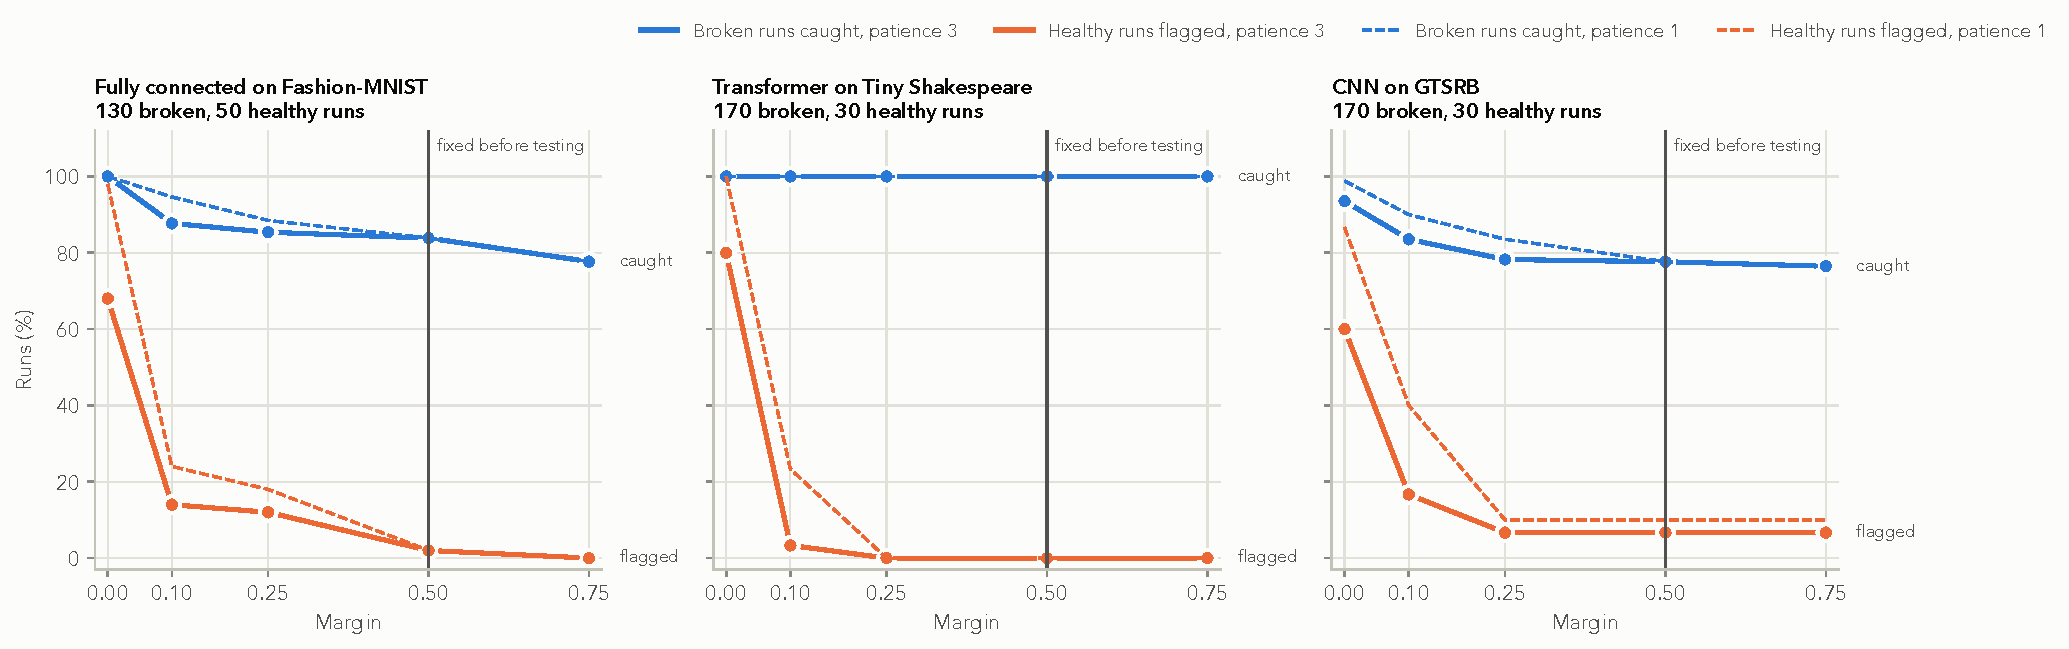
\includegraphics[width=\linewidth]{figures/tradeoff.pdf}
\caption{Broken runs caught and healthy runs flagged as the margin changes, at floor 0.05. Solid lines use patience 3 and dashed lines patience 1.}
\label{fig:tradeoff}
\end{figure}


\begin{figure}[t]
\centering
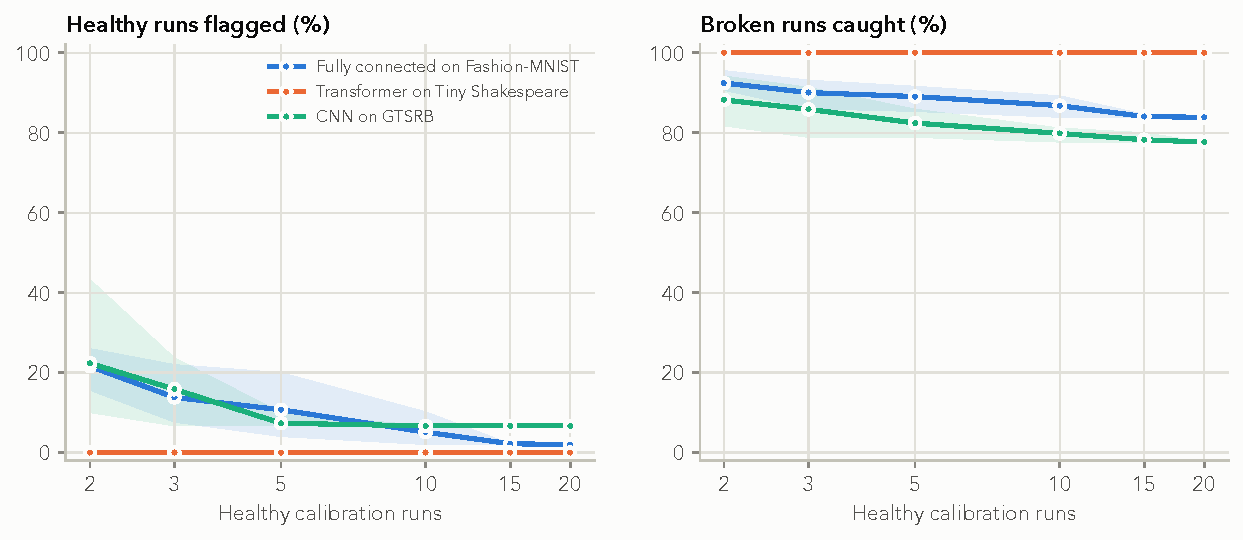
\includegraphics[width=\linewidth]{figures/calibration_size.pdf}
\caption{False alarms and broken runs caught when the healthy range is built from fewer calibration runs.}
\label{fig:calibration_size}
\end{figure}


\subsection{Cost}

Monitoring added 11.6\% for the fully connected network, 5.8\% for the transformer, 2.2\% for the CNN, measured on fresh healthy runs on one CPU thread. Most of the cost is the gradient norm, read after every batch, and the probe batch, run once per epoch, so smaller networks with cheap epochs pay the largest share. Stopping each broken run at LHD's alarm would have saved 70\% of its training on average. All runs together took 94 hours of CPU time on one laptop.

\section{Discussion and Limitations}

The results support the hypothesis for planted faults. Per layer signals exposed a broken layer within the first few epochs, usually before the accuracy curve showed anything, and LHD rarely flagged healthy runs. They also show where the idea's value lies. A frozen layer is caught just as well, and sooner, by a check for weights that never change, so LHD's contribution there is only that the same rules cover it. For dead units, a range measured on healthy runs of the same network did better than every fixed threshold tested, including the defaults of three existing tools.

Several limits apply. The faults were planted to show up in the signals LHD measures, so detection and diagnosis rates describe how well LHD separates these faults from normal variation, not how often it would catch bugs found in the wild. Many planted faults cost less than one point of accuracy, so stopping those runs saves compute on runs that would have produced a nearly normal model. LHD misses dead units in layers where healthy runs already lose many units, because the healthy range treats that loss as normal. The healthy range needs about 10 to 20 healthy runs of the same network, which costs more than LHD can save for a model trained only once, and it assumes those runs are themselves healthy. The networks are small, trained for 15 to 20 epochs on a laptop CPU, and the transformer reaches only about 37\% next character accuracy. Large networks, long runs, other optimizers, and GPU training were not tested.

\section{Conclusion}

This work presented LHD, a monitor that compares four per layer signals with ranges measured on healthy runs of the same network and stops a run when one stays out of range. On 645 runs across three networks, LHD caught most planted frozen layers and dead units within three epochs, named the right layer almost every time, and rarely flagged healthy runs. Its clearest advantage over existing tools is for dead units, where a healthy range per layer avoided the misses and false alarms of fixed thresholds. Testing LHD on real bugs collected from training code is the next step.

\section*{Code and data}

The code, every saved run, and the tables behind each number are at \url{https://github.com/sohan-bhat/lhd}.


\begin{thebibliography}{99}

\bibitem[Amazon Web Services(n.d.a)]{aws_rules}
Amazon Web Services (n.d.a).
\newblock List of Debugger built-in rules.
\newblock Amazon SageMaker AI Developer Guide.
\newblock \url{https://docs.aws.amazon.com/sagemaker/latest/dg/debugger-built-in-rules.html}

\bibitem[Amazon Web Services(n.d.b)]{aws_actions}
Amazon Web Services (n.d.b).
\newblock Use Debugger built-in actions for rules.
\newblock Amazon SageMaker AI Developer Guide.
\newblock \url{https://docs.aws.amazon.com/sagemaker/latest/dg/debugger-built-in-actions.html}

\bibitem[Biewald(2020)]{biewald2020}
Biewald, L. (2020).
\newblock Experiment tracking with Weights and Biases.
\newblock Software available from wandb.com.
\newblock \url{https://www.wandb.com/}

\bibitem[Chwilczy\'nski et~al.(2024)]{chwilczynski2024}
Chwilczy\'nski, S., Tr\k{e}bacz, K., Cyganik, K., Ma\l{}ecki, M., and Brzezinski, D. (2024).
\newblock ART: Actually Robust Training.
\newblock In \emph{Machine Learning and Knowledge Discovery in Databases. Research Track and Demo Track (ECML PKDD 2024)}, Lecture Notes in Computer Science, vol.~14948, pp.~374--378. Springer, Cham.
\newblock \url{https://doi.org/10.1007/978-3-031-70371-3_23}. Preprint: arXiv:2408.16285.

\bibitem[CS231n(n.d.)]{cs231n}
CS231n (n.d.).
\newblock Neural networks part 3: Learning and evaluation.
\newblock Course notes for CS231n, Stanford University.
\newblock \url{https://cs231n.github.io/neural-networks-3/}

\bibitem[Groeger(n.d.)]{groeger_wandbcallbacks}
Groeger, F. (n.d.).
\newblock wandb-callbacks: Additional callbacks for Weights \& Biases.
\newblock GitHub repository.
\newblock \url{https://github.com/FabianGroeger96/wandb-callbacks}

\bibitem[Karpathy(2019)]{karpathy2019}
Karpathy, A. (2019).
\newblock A recipe for training neural networks.
\newblock Blog post, April 25, 2019.
\newblock \url{https://karpathy.github.io/2019/04/25/recipe/}

\bibitem[Stallkamp et~al.(2012)]{stallkamp2012}
Stallkamp, J., Schlipsing, M., Salmen, J., and Igel, C. (2012).
\newblock Man vs.\ computer: Benchmarking machine learning algorithms for traffic sign recognition.
\newblock \emph{Neural Networks}, 32:323--332.
\newblock \url{https://doi.org/10.1016/j.neunet.2012.02.016}

\bibitem[Wardat et~al.(2022)]{wardat2022}
Wardat, M., Cruz, B.~D., Le, W., and Rajan, H. (2022).
\newblock DeepDiagnosis: Automatically diagnosing faults and recommending actionable fixes in deep learning programs.
\newblock In \emph{Proceedings of the 44th International Conference on Software Engineering (ICSE 2022)}, pp.~561--572. ACM, New York.
\newblock \url{https://doi.org/10.1145/3510003.3510071}. Preprint: arXiv:2112.04036.

\bibitem[Zhang et~al.(2021)]{zhang2021}
Zhang, X., Zhai, J., Ma, S., and Shen, C. (2021).
\newblock AUTOTRAINER: An automatic DNN training problem detection and repair system.
\newblock In \emph{2021 IEEE/ACM 43rd International Conference on Software Engineering (ICSE)}, pp.~359--371. IEEE.
\newblock \url{https://doi.org/10.1109/ICSE43902.2021.00043}

\end{thebibliography}


\end{document}
